\documentclass[a4paper, 10pt]{article}

% Typography & Font Handling
%\usepackage[utf8]{inputenc}
\usepackage[T1]{fontenc}
\usepackage{lmodern}
\usepackage{microtype}
\usepackage{fontspec}
\usepackage{sectsty}
\usepackage{fixltx2e}
\usepackage{titlesec}

% Fonts
%\usepackage{garamondlibre}
\setmainfont{Garamond Libre}  % Serif
\setsansfont{TeX Gyre Heros}    % Sans
\setmonofont{TeX Gyre Cursor}  % Mono

% Mathematics
\usepackage{amsmath}
\usepackage{amssymb}
\usepackage{mathtools}

% Numbers
\usepackage{siunitx}
\sisetup{
    detect-all,   % detects the surrounding font
    detect-family,
    detect-shape,
    detect-weight
}

% Lists
\usepackage{enumitem}

% Tables
\usepackage{booktabs}
\usepackage{array}
\usepackage{tabularx}
\newcolumntype{Y}{>{\raggedright\arraybackslash}X}

% Graphics
\usepackage{graphicx}
\usepackage{float}

% Figures
\usepackage{subcaption}
\usepackage{wrapfig}

% Circuits
\usepackage{circuitikz}

% Code Listings
\usepackage{listings}

% Layout & Page Formatting
\usepackage{geometry}
\usepackage{fancyhdr}
%\usepackage{indentfirst}
\usepackage{parskip}
% References
\usepackage{hyperref}
\usepackage{cleveref}

%\usepackage{lipsum}

%============================================
\geometry{
headheight=25pt,
top=1in,
bottom=1in,
left=0.5in,
right=0.5in
}
\title{ELEC ENG 2411 Ex: 2\vspace{5em}
}
\author{
	{\Large Prepared by:}\\
	Lucas Rufkahr\vspace{5em}\\
	{\Large In Collaboration with:}\\
	Aiden Burns\vspace{5em}\\
	{\Large Submitted to:}\\
	Sokrat Aldarmini\vspace{5em}\\
	{\Large Submitted on:}\\
	\today
}
\date{}

\titleformat*{\section}{\Large\bfseries\sffamily}
\renewcommand{\thesection}{\arabic{section}}
\titleformat*{\subsection}{\large\bfseries\sffamily}
\renewcommand{\thesubsection}{\thesection.\Alph{subsection}}
\titleformat*{\subsubsection}{\itshape\sffamily}
\renewcommand{\thesubsubsection}{\thesubsection.\roman{subsubsection}}

\begin{document}
\setcounter{secnumdepth}{4}
\pagestyle{fancy}
\fancyhead[L]{Lucas Rufkahr, Aiden Burns}
\fancyhead[C]{Experiment 2}
\fancyhead[R]{EE2411 --- Section 305\\\today}
\maketitle
\thispagestyle{empty}
%========================
\pagebreak
\section*{Part 4 Step 1}
We selected our base components for our RC circuit and found our components were within tolerance. The internal resistance was combined with our resistor for a total resistance of $1041.3\si{\ohm}$.
\begin{table}[H]
        \centering
        \begin{tabularx}{0.7\linewidth}{YYYY}
		$R$ (\si{\ohm}) & $C$ (F) & $R_{in}$ (\si{\ohm}) & $R' = R_{in} + R$ (\si{\ohm})\\
		$991.3$ & $0.000000112$ & $50$ & $1041.3$\\
        \end{tabularx}
	\caption{Values for component pieces and total circuit resistance.}
	\label{tab:component_values}
\end{table}
\section*{Part 4 Step 3}
%
% Describe the behavior of the RC circuit with respect to different frequency sinusoids,
% paying attention to amplitude and phase. Is this a low-pass or high-pass filter?
%
With a $100$Hz sinusoid, we find that the effect of the system on input signal is negligible with no noticeable difference on phase shift and $V_{pp}$ as seen on channel 2 in figure \ref{fig:scope_100hz_sinusoid}. As the frequency of channel 1 increases, we see that the phase shift and amplitude of channel 2 change drastically. A $1$kHz sinusoid results in a phase shift of $-29.52^{\circ}$ and an amplitude of $1.84V$ shown in figure \ref{fig:scope_1khz_sinusoid}. A $10$kHz sinusoid results in a phase shift of $-74.02^{\circ}$ and an amplitude of $336mV$ shown in figure \ref{fig:scope_10khz_sinusoid}. Based on these effects, we can consider this circuit to be a low pass filter. We can determine this by looking at figure \ref{fig:scope_10khz_sinusoid} where the output signal appears to be increasing as the input signal decreases. This indicates that the circuit is passing ``low'' input.
\begin{figure}[H]
        \centering
        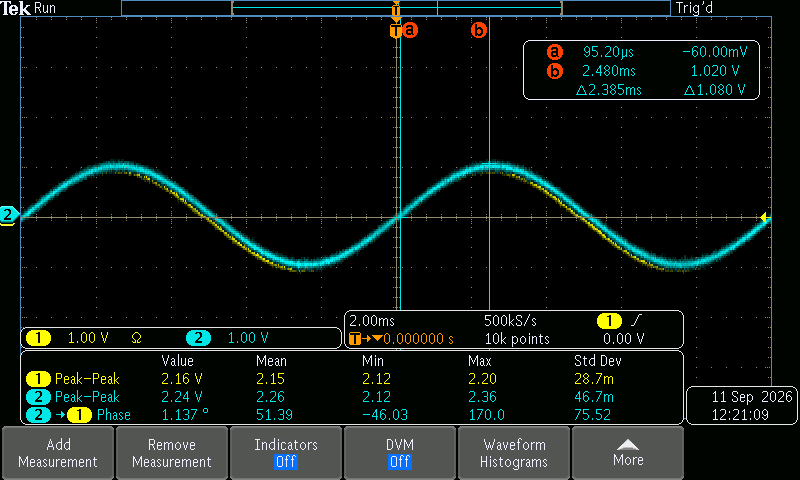
\includegraphics[scale=0.5]{./assets/scope/100HZ_sinusoid.png}
        \caption{100Hz Sinusoid}
        \label{fig:scope_100hz_sinusoid}
\end{figure}
\begin{figure}[H]
        \centering
        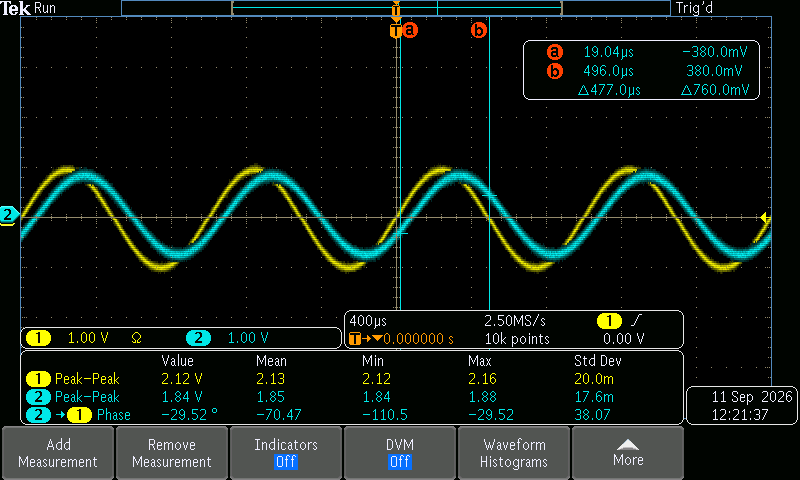
\includegraphics[scale=0.5]{./assets/scope/1KHZ_sinusoid.png}
        \caption{1kHz Sinusoid}
        \label{fig:scope_1khz_sinusoid}
\end{figure}
\begin{figure}[H]
	\centering
        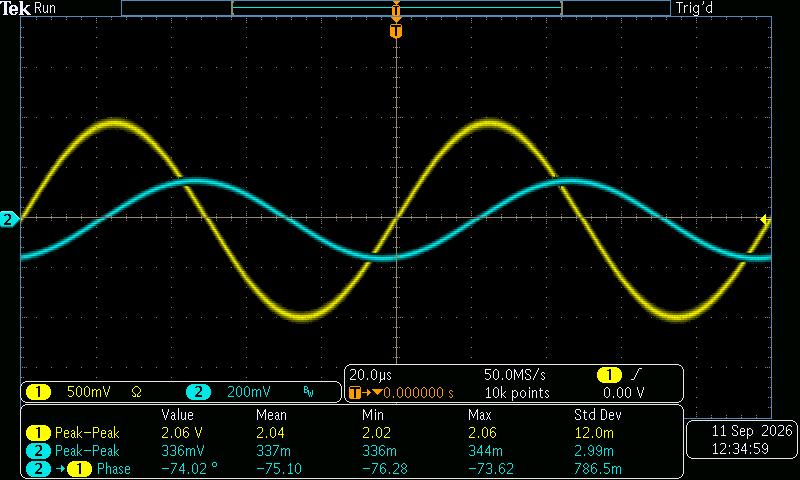
\includegraphics[scale=0.5]{./assets/scope/10KHZ_sinusoid.png}
        \caption{10kHz Sinusoid}
        \label{fig:scope_10khz_sinusoid}
\end{figure}
\begin{table}[H]
	\centering
	\begin{tabularx}{0.7\linewidth}{YYYY}
		Frequency (kHz) & Channel 1 $V_{pp}$ & Channel 2 $V_{pp}$ & $\theta_{2,1}^{\circ}$ \\
		$0.100$ & $2.16$ & $2.24$ & $1.137$ \\
		$1.0$ & $2.12$ & $1.84$ & $-29.52$ \\
		$10.0$ & $2.06$ & $0.336$ & $-74.02$ \\
	\end{tabularx}
	\caption{Increasing frequency values with associated channel $V_{pp}$ and phase shift.}
	\label{tab:scope_sinusoid_measurements}
\end{table}
\section*{Part 4 Step 4}
To find the time constant we consider our system where $x(t)$ is the input and $y(t)$ is the output.
\begin{equation*}
	\frac{dy(t)}{dt} + \frac{1}{RC}y(t) = \frac{1}{RC}x(t)
\end{equation*}
We assume the form $y(t) = Ae^{\lambda_{1}t} + Be^{\lambda_{2}t}$. We then write out the characteristic equation and solve for $\lambda$. Then we substitute $\lambda$ into our solution.
\begin{align*}
	\lambda + \frac{1}{RC} & = 0\\
	\lambda_{1} & = -\frac{1}{RC}\\
	y(t) & = Ae^{-\frac{t}{RC}}
\end{align*}
From our solution, we find the time constant $\tau = RC$. Using experimental values for $R$ and $C$ we find the experimental time constant should be $1.17\times10^{-4}$. The ratio of the rise time over the time constant is $1.12$.
\begin{table}[H]
	\centering
	\begin{tabularx}{0.7\linewidth}{YYY}
		Rise Time ($\mu s$), $t_r$ & Time constant ($\mu s$), $\tau$ & $\frac{t_r}{\tau}$\\
		$131.3$ & $117$ & $1.12$
	\end{tabularx}
	\caption{Experimental rise time, time constant, and ratio of rise time and time constant.}
	\label{tab:scope_rise_time}
\end{table}
\section*{Part 4 Step 5}
%
% Describe the behavior of the RC circuit with respect to different frequency square waves.
% Why does the wave distort at the output? Is there a relationship to the time constant?
%
Both the 100Hz signal and the 1kHz signal show no distortion of the output signal and we see on both figure \ref{fig:scope_100hz_square} and figure \ref{fig:scope_1khz_square} have the same signals within margin of error. The 10kHz signal shown in figure \ref{fig:scope_10khz_square} shows drastic distortion. We see that $V_{pp}$ of channel 2 is $600mV$ with the start of the signal showing above the low signal of channel 1 indicating that the capacitor does not have enough time to discharge before a high signal enters the system so there is still residual potential in the capacitor. The capacitor also does not have enough time to charge before the high signal leaves and does not reach the full amplitude of the input. Given that our time constant is the time it takes to reach 63\% of the full potential, a 10kHz square has a period of $100\mu s$ and a high or low signal has a time of $50\mu s$, we can determine that our signal is too ``quick'' since $50\mu s < 117\mu s$. 
\begin{figure}[H]
        \centering
        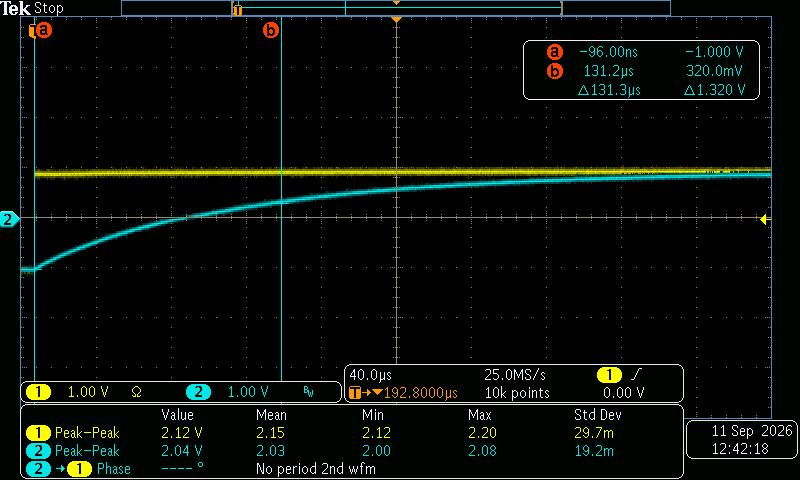
\includegraphics[scale=0.5]{./assets/scope/100HZ_square.png}
        \caption{100Hz Square}
        \label{fig:scope_100hz_square}
\end{figure}
\begin{figure}[H]
        \centering
        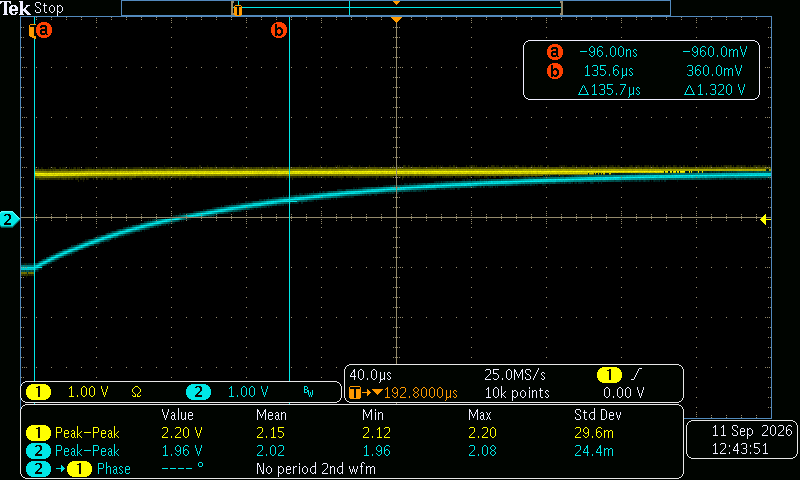
\includegraphics[scale=0.5]{./assets/scope/1KHZ_square.png}
        \caption{1kHz Square}
        \label{fig:scope_1khz_square}
\end{figure}
\begin{figure}[H]
	\centering
        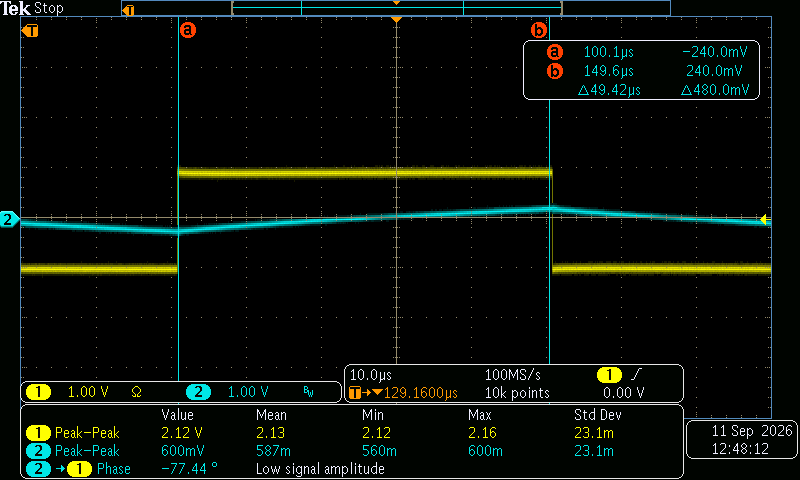
\includegraphics[scale=0.5]{./assets/scope/10KHZ_square.png}
        \caption{10kHz Square}
        \label{fig:scope_10khz_square}
\end{figure}
\begin{table}[H]
	\centering
	\begin{tabularx}{0.7\linewidth}{YYY}
		Frequency (kHz) & Channel 1 $V_{pp}$ & Channel 2 $V_{pp}$ \\
		$0.100$ & $2.12$ & $2.04$ \\
		$1.0$ & $2.20$ & $1.96$ \\
		$10.0$ & $2.12$ & $0.600$ \\
	\end{tabularx}
	\caption{Frequency of input signal and voltage peaks for input and output signals.}
	\label{tab:scope_square_measurements}
\end{table}
\section*{Part 5 Step 6}
%
% Compare the behavior of the Simulink model with that of the experimental setup. Does
% it behave as a filter? Are the changes in amplitude and phase with increasing frequency
% comparable?
%
We use MATLAB Simulink software to model our system on our computer. We ran our simulation with a runtime of $3/freq$ so each runs for three periods. To find the phase shift, we take the time change between signal peaks and multiply it by $2\pi$ over the period. We found that our simulation appears to behave as a low pass filter with behavior that increases as the frequency increases. The changes in amplitude and phase is comparable to that of our experimental results.
\begin{equation*}
	\Delta\theta = \Delta t \frac{2\pi}{T}
\end{equation*}
\begin{figure}[H]
        \centering
        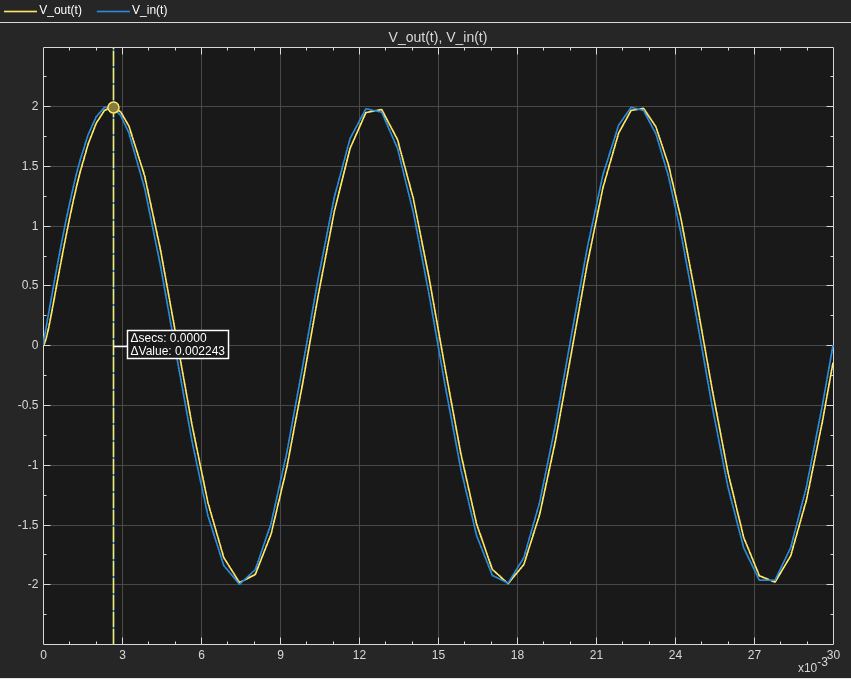
\includegraphics[scale=0.4]{./assets/simulink/100HZ_sinusoid.png}
        \caption{100Hz Sinusoid}
        \label{fig:simulink_100hz_sinusoid}
\end{figure}
\begin{figure}[H]
        \centering
        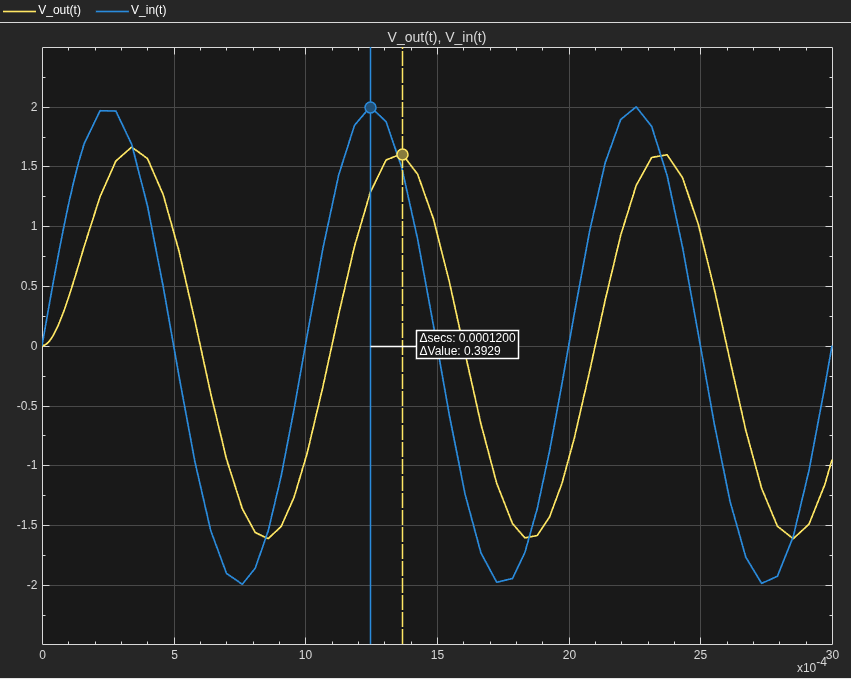
\includegraphics[scale=0.4]{./assets/simulink/1KHZ_sinusoid.png}
        \caption{1kHz Sinusoid}
        \label{fig:simulink_1khz_sinusoid}
\end{figure}
\begin{figure}[H]
	\centering
        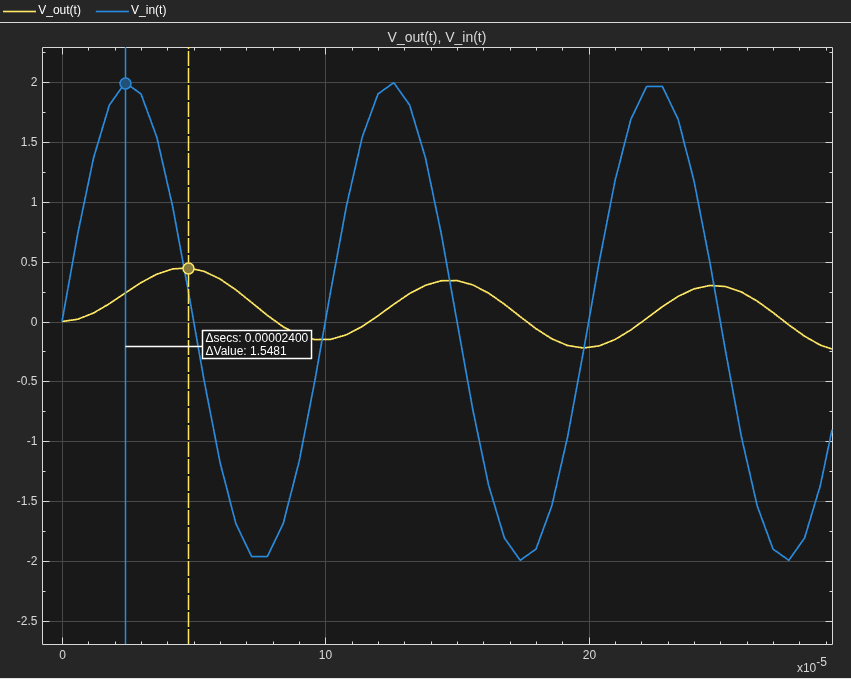
\includegraphics[scale=0.4]{./assets/simulink/10KHZ_sinusoid.png}
        \caption{10kHz Sinusoid}
        \label{fig:simulink_10khz_sinusoid}
\end{figure}
\begin{table}[H]
	\centering
	\begin{tabularx}{0.7\linewidth}{YYYY}
		Frequency (kHz) & $V_{in,pp}$ & $V_{o,pp}$ & $\Delta\theta (rad)$ \\
		$0.100$ & $1.996$ & $1.994$ & $0$ \\
		$1.0$ & $1.996$ & $1.661$ & $0.75$ \\
		$10.0$ & $1.996$ & $0.449$ & $1.51$ \\
	\end{tabularx}
	\caption{Theoretically modeled frequencies with their associated $V_{pp}$ and phase shift.}
	\label{tab:simulink_sinusoid_measurements}
\end{table}
\section*{Part 5 Step 7}
%
% Calculate percent error with the hardware values.
%
Using the standard percent error formula, we found the percent error of our rise time to be $1.29\%$. We also found the percent error of our ratio to be $1.79\%$.
\begin{table}[H]
	\centering
	\begin{tabularx}{0.7\linewidth}{YYY}
		Rise Time ($\mu s$), $t_r$ & Time constant ($\mu s$), $\tau$ & $\frac{t_r}{\tau}$\\
		133.0 & 117 & 1.14
	\end{tabularx}
	\caption{Theoretically modeled rise time, time constant, and ratio of rise time over time constant.}
	\label{tab:simulink_rise_time}
\end{table}
\section*{Part 5 Step 8}
%
% Compare the behavior of the Simulink model with that of the experimental setup. Does
% it have the same effects on the input signals? Are the changes in amplitude and phase
% with increasing frequency comparable (within 10%)?
%
We use MATLAB Simulink software to model our system on our computer. We ran our simulation with a runtime of $3/freq$ so each runs for three periods. We found that the Simulink output matches that of our physical experiment though the behavior is more pronounced in the simulation.

For our sinusoidal model, we found that at the 100Hz signal the peak to peak voltages and phase shift are roughly the same. For the 1kHz signal, the peak to peak voltages in the experimental case are roughly 10\% higher than the model. The phase shift in our experiment is half what is shown in the model. For the 10kHz signal, the peak to peak voltages in the experimental case are roughly 25\% higher than the model. The phase shift is also roughly 14\% higher in the experimental case than the model.

For our square model, we found that at the 100Hz signal, the peak to peak voltages were roughly the same. For the 1kHz signal, the peak to peak voltages were also roughly the same. For the 10kHz signal, the voltage peaks for the output were roughly 30\% higher in the experiment compared to the model.
\begin{figure}[H]
        \centering
        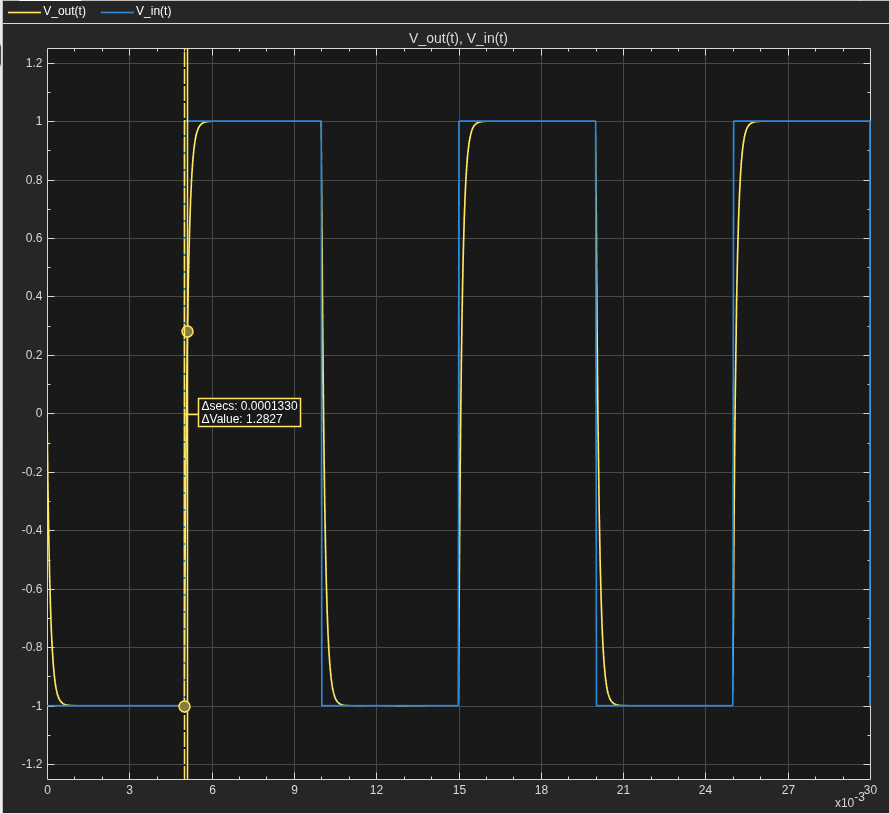
\includegraphics[scale=0.4]{./assets/simulink/100HZ_square.png}
        \caption{100Hz Square}
        \label{fig:simulink_100hz_square}
\end{figure}
\begin{figure}[H]
        \centering
        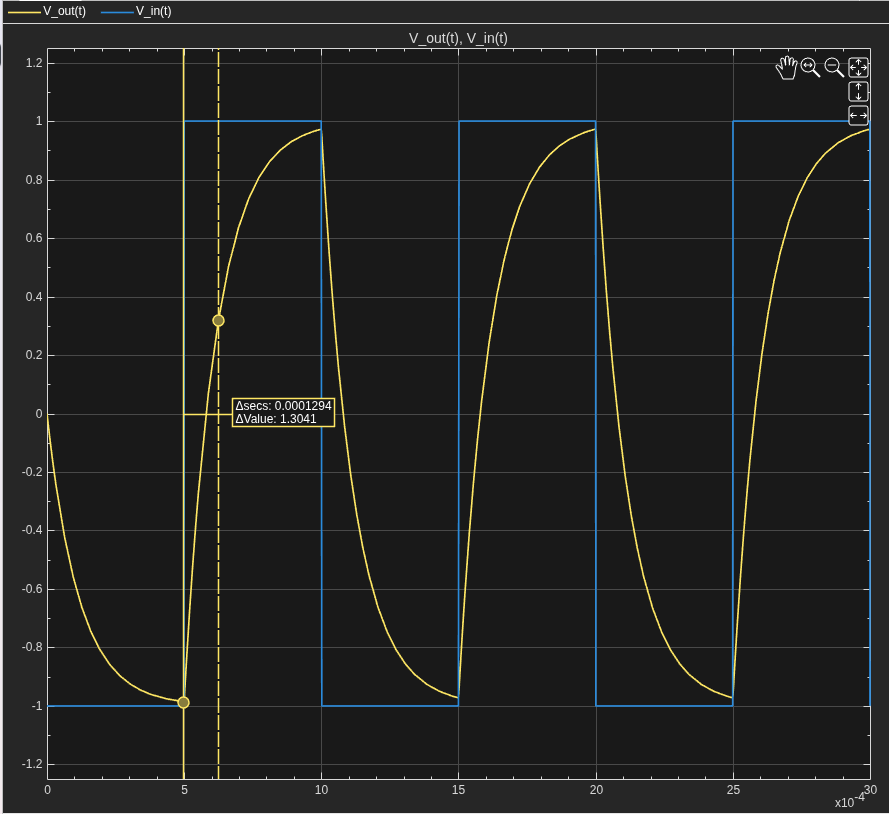
\includegraphics[scale=0.4]{./assets/simulink/1KHZ_square.png}
        \caption{1kHz Square}
        \label{fig:simulink_1khz_square}
\end{figure}
\begin{figure}[H]
	\centering
        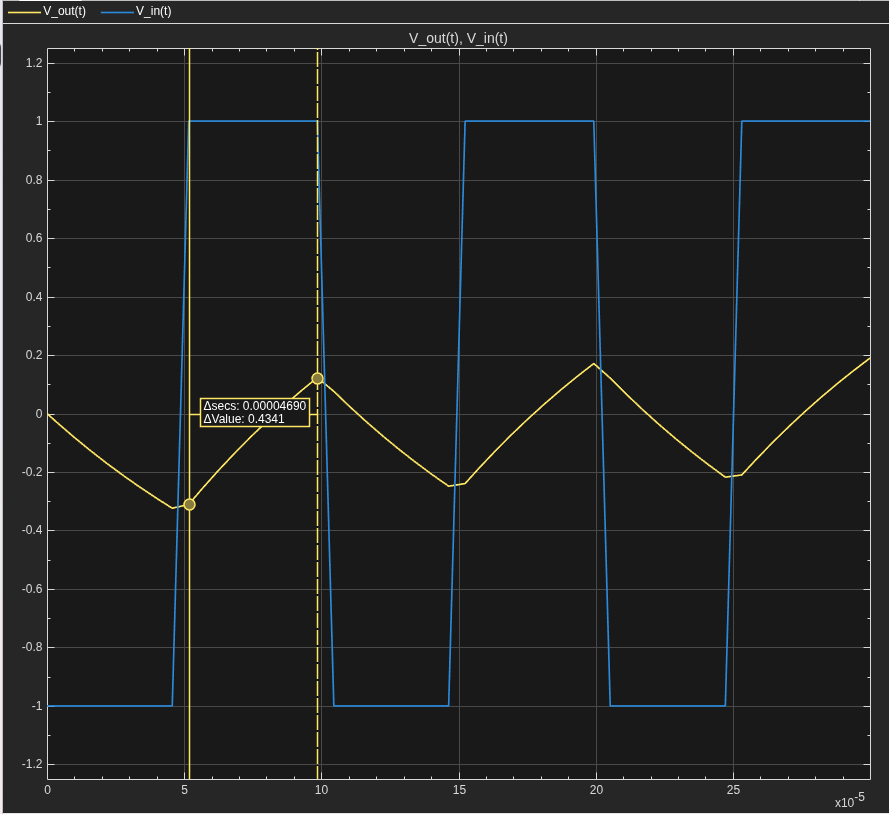
\includegraphics[scale=0.4]{./assets/simulink/10KHZ_square.png}
        \caption{10kHz Square}
        \label{fig:simulink_10khz_square}
\end{figure}
\begin{table}[H]
	\centering
	\begin{tabularx}{0.7\linewidth}{YYY}
		Frequency (kHz) & Channel 1 $V_{pp}$ & Channel 2 $V_{pp}$ \\
		$0.100$ & $2.0$ & $2.0$ \\
		$1.0$ & $2.0$ & $1.94$ \\
		$10.0$ & $2.0$ & $0.43$ \\
	\end{tabularx}
	\caption{Theoretically modeled frequency of input signal and voltage peaks for input and output signals.}
	\label{tab:simulink_square_measurements}
\end{table}
\end{document}
